\documentclass[border=6pt]{standalone}
% Shared preamble for web figures.  Each figure is a standalone .tex that
% \input's this file; scripts/make-figures.sh turns it into an SVG.
\usepackage[T1]{fontenc}
\usepackage{helvet}
\renewcommand{\familydefault}{\sfdefault}
\usepackage{tikz}
\usetikzlibrary{decorations.pathreplacing}
% axis numbers in the text font, not math italic
\pgfkeys{/pgf/number format/.cd,assume math mode=true,1000 sep={}}

% dot plot: \dotplot{min}{max}{value/count,...}{axis label}
\newcommand{\dotplot}[4]{%
\begin{tikzpicture}[x=0.9cm,y=0.33cm]
  \draw[thick] (#1-0.5,0) -- (#2+0.5,0);
  \foreach \t in {#1,...,#2} {\draw (\t,0.25) -- (\t,-0.25) node[below] {\t};}
  \foreach \v/\c in {#3} {\ifnum\c>0 \foreach \k in {1,...,\c} {\fill (\v,\k*1.15) circle (0.16cm);}\fi}
  \node at ({(#1+#2)/2},-2.3) {#4};
\end{tikzpicture}}

% shape sketch histogram (12 bins): \shapehist{heights}{label}
\newcommand{\shapehist}[2]{%
  \foreach \h [count=\i from 0] in {#1} \draw[fill=gray!30] (\i,0) rectangle (\i+1,\h);
  \draw (-0.3,0) -- (12.3,0);
  \node[font=\bfseries] at (6,-2.6) {#2};}
\newcommand{\meanmark}[1]{\fill (#1,0) -- ++(-0.3,-0.75) -- ++(0.6,0) -- cycle;}
\newcommand{\medmark}[2]{\draw[very thick,dashed] (#1,0) -- (#1,#2);}

% number line with minor ticks: \nline{min}{max}{label step}{axis label}
\newcommand{\nline}[4]{%
  \draw[thick] (#1-0.5,0) -- (#2+0.5,0);
  \foreach \t in {#1,...,#2} \draw (\t,0.12) -- (\t,-0.12);
  \pgfmathtruncatemacro{\nxt}{#1+#3}
  \foreach \t in {#1,\nxt,...,#2} \draw (\t,0.2) -- (\t,-0.2) node[below] {\t};
  \node at ({(#1+#2)/2},-0.95) {#4};}
% box plot above the line: \bplot{min}{Q1}{med}{Q3}{max}
\newcommand{\bplot}[5]{%
  \draw[thick] (#1,1.0) -- (#2,1.0);
  \draw[thick] (#4,1.0) -- (#5,1.0);
  \draw[thick] (#1,0.75) -- (#1,1.25);
  \draw[thick] (#5,0.75) -- (#5,1.25);
  \draw[thick,fill=gray!20] (#2,0.55) rectangle (#4,1.45);
  \draw[very thick] (#3,0.55) -- (#3,1.45);}

% ---- added for 1.4 onward ----
% axis on y=0: \axis{min}{max}{label step}{tick step}{axis label}
\newcommand{\axis}[5]{%
  \draw[thick] (#1,0) -- (#2,0);
  \pgfmathsetmacro{\axT}{#1+#4}\foreach \t in {#1,\axT,...,#2} \draw (\t,0.1) -- (\t,-0.1);
  \pgfmathsetmacro{\axL}{#1+#3}\foreach \t in {#1,\axL,...,#2}
    \draw (\t,0.18) -- (\t,-0.18) node[below] {\pgfmathprintnumber{\t}};
  \node at ({(#1+#2)/2},-0.95) {#5};}
% box plot centred at height y: \bplotat{y}{min}{Q1}{med}{Q3}{max}
\newcommand{\bplotat}[6]{%
  \draw[thick] (#2,#1) -- (#3,#1);
  \draw[thick] (#5,#1) -- (#6,#1);
  \draw[thick] (#2,#1-0.22) -- (#2,#1+0.22);
  \draw[thick] (#6,#1-0.22) -- (#6,#1+0.22);
  \draw[thick,fill=gray!20] (#3,#1-0.42) rectangle (#5,#1+0.42);
  \draw[very thick] (#4,#1-0.42) -- (#4,#1+0.42);}
% an outlier dot: \outlier{x}{y}
\newcommand{\outlier}[2]{\fill (#1,#2) circle (2.4pt);}

\begin{document}
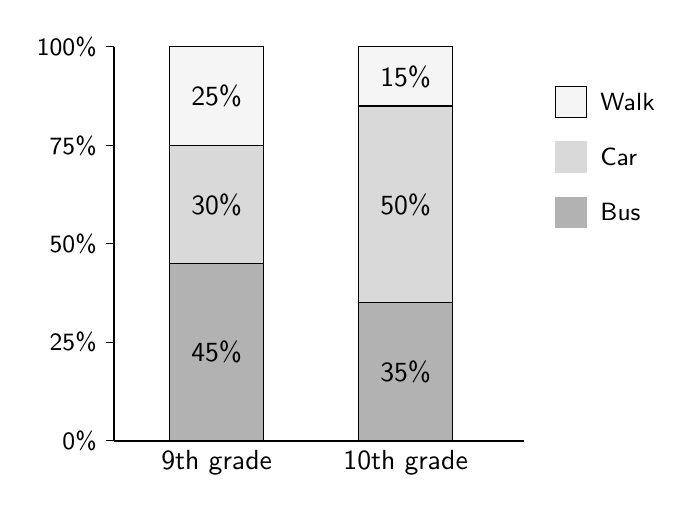
\begin{tikzpicture}[x=1cm,y=0.05cm]
  \draw[thick] (0,0) -- (5.2,0); \draw[thick] (0,0) -- (0,100);
  \foreach \p in {0,25,50,75,100} {\draw (0,\p) -- (-0.1,\p) node[left,font=\small] {\p\%};}
  % 9th: bus 45, car 30, walk 25
  \fill[gray!60] (0.7,0) rectangle (1.9,45); \fill[gray!30] (0.7,45) rectangle (1.9,75); \fill[gray!8] (0.7,75) rectangle (1.9,100);
  \draw (0.7,0) rectangle (1.9,100); \draw (0.7,45) -- (1.9,45); \draw (0.7,75) -- (1.9,75);
  \node at (1.3,22.5) {45\%}; \node at (1.3,60) {30\%}; \node at (1.3,87.5) {25\%};
  % 10th: bus 35, car 50, walk 15
  \fill[gray!60] (3.1,0) rectangle (4.3,35); \fill[gray!30] (3.1,35) rectangle (4.3,85); \fill[gray!8] (3.1,85) rectangle (4.3,100);
  \draw (3.1,0) rectangle (4.3,100); \draw (3.1,35) -- (4.3,35); \draw (3.1,85) -- (4.3,85);
  \node at (3.7,17.5) {35\%}; \node at (3.7,60) {50\%}; \node at (3.7,92.5) {15\%};
  \node[below] at (1.3,0) {9th grade}; \node[below] at (3.7,0) {10th grade};
  \fill[gray!8] (5.6,82) rectangle (6.0,90); \draw (5.6,82) rectangle (6.0,90); \node[right,font=\small] at (6.05,86) {Walk};
  \fill[gray!30] (5.6,68) rectangle (6.0,76); \node[right,font=\small] at (6.05,72) {Car};
  \fill[gray!60] (5.6,54) rectangle (6.0,62); \node[right,font=\small] at (6.05,58) {Bus};
\end{tikzpicture}
\end{document}
